\documentclass{beamer}
\usepackage{styles/mystyle}
%----------------------------------------------------------------------------------------
%	TITLE PAGE
%----------------------------------------------------------------------------------------
\title[SaSSLR]{Software as Storytelling: a systematic literature review}

\subtitle{\small P. Ciancarini, M. Farina, O. Okonicha, M. Smirnova, G. Succi}
\author{presentazione a cura di Federico Licastro}

\begin{document}

\begin{frame}
  \titlepage
\end{frame}
%---------------------------------------------
\begin{frame}{\centerline{Cos'è lo storytelling?}}

Lo storytelling rappresenta quella pratica tramite cui l'uomo ha potuto scambiarsi idee, credenze ed esperienze fin dalla preistoria .

   \vspace{0.5cm}
   
Le origini visuali di questa pratica \cite{feliks2011prehistory}, che consiste nel raccontare una storia, si sono trasformate nel corso dei secoli verso un sistema di narrazione coerente e sistematizzato. 

      \vspace{0.5cm}
      
      \begin{figure}[H]
  \begin{tabulary}{\textwidth}{m{5.5cm} m{5.5cm}}
        Secondo \citeauthor{Ciriello2017ProtoStory}, una storia \'e un resoconto di azioni raccolte da eventi, sia reali sia di fantasia. & 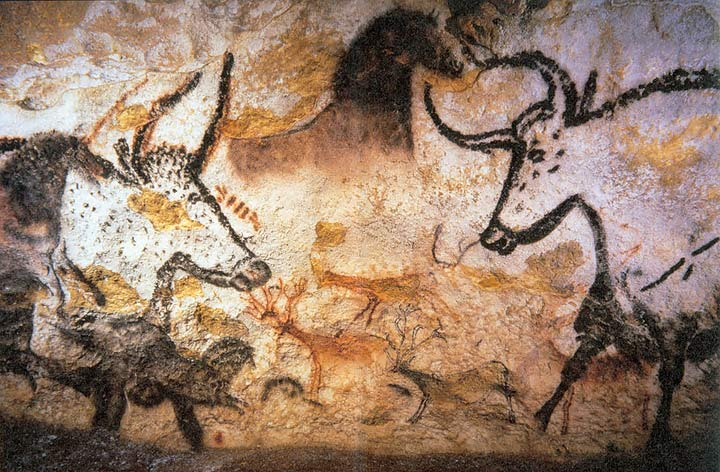
\includegraphics[width=0.4\textwidth]{images/img-1.jpg}
            \caption{Grotte di Lascaux}
        \\
    \end{tabulary}
    \end{figure}

%\begin{flushright}
%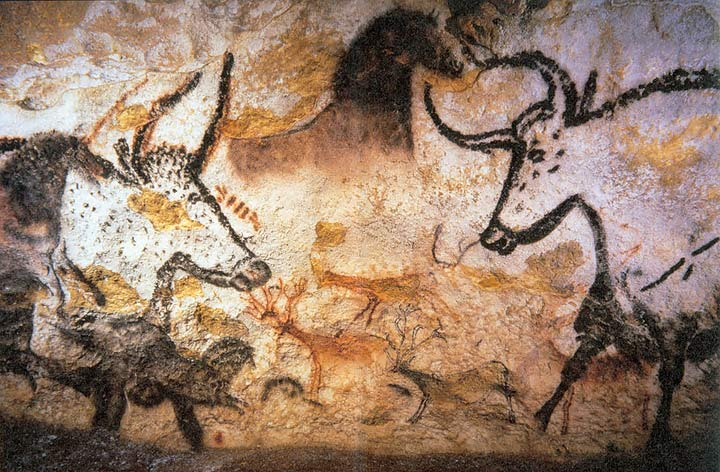
\includegraphics[width=0.5\textwidth]{images/img-1.jpg}
%\end{flushright}

\end{frame}
%=============================================

%---------------------------------------------
\begin{frame}{\centerline{Galassia interdisciplinare dello storytelling}}
    \begin{tikzpicture}[remember picture, overlay,
        % Definisci gli stili dei cerchi
        bigcircle/.style={circle, draw=#1, fill=#1!20, minimum size=2cm, align=center},
        smallcircle/.style={circle, draw=#1, fill=#1!20, minimum size=1cm, align=center}
    ]
        % Posizioni dei cerchi
        \node[bigcircle=myred] (oral) at ([yshift=-1.8cm,xshift=-4cm]current page.center) {Oral storytelling};
        \node[bigcircle=myyellow] (written) at ([yshift=-2.6cm,xshift=-0.5cm]current page.center) {Written storytelling};
        \node[smallcircle=green] (artistic) at ([yshift=-1.6cm,xshift=3cm]current page.center) {Artistic \\performances};
        \node[smallcircle=orange] (visual) at ([yshift=-3cm,xshift=5cm]current page.center) {Visual \\storytelling};
        \node[smallcircle=brown] (digital) at ([yshift=2cm,xshift=-4cm]current page.center) {Digital \\storytelling};
        \node[smallcircle=blue] (virtual) at ([yshift=2cm,xshift=-1cm]current page.center) {Virtual\\reality \\storytelling};
        \node[smallcircle=magenta] (transmedia) at ([yshift=2cm,xshift=2cm]current page.center) {Transmedia \\storytelling};
    \end{tikzpicture}
    
    \begin{center}
        Quale tipologia di storytelling risulta di maggior interesse nel SD?
    \end{center}
\end{frame}
%=============================================

\begin{frame}{\centerline{Cos'è il software development?}}
\setstretch{1.5}
\citet{kernighan1976software} hanno definito lo sviluppo software come "\textit{il processo tramite cui \textcolor{myyellow}{\textbf{i bisogni dell'utilizzatore sono tradotti in un prodotto software}}. Il processo coinvolge  \textcolor{myred}{\textbf{la traduzione dei bisogni degli utenti in requisiti software}},  \textbf{la trasformazione dei requisiti software in progettazione},  l'implementazione della progettazione nel codice, il testing del codice e, talvolta, l'installazione e il controllo del software per l'utilizzo operativo}"
\end{frame}

\begin{frame}{\centerline{Galassia dello sviluppo software: due pianeti}}
\begin{table}[H]
\begin{tabulary}{\textwidth}{m{5cm} m{5cm}}
\begin{tikzpicture}
\fill[myred] (0,0) circle (2.7cm);
\node[text=white, font=\fontsize{9}{9}\selectfont] at (0,1.4) {\shortstack{Waterfall\\\\azioni prefissate e rigide}}
\node[text=white, font=\fontsize{7}{9}\selectfont] at (0,-0.3)
{\shortstack{System Development Life Cycle\\SDLC models}}
\node[text=white, font=\fontsize{7}{9}\selectfont] at (0,-1.4)
{\shortstack{\citeauthor{Isaias2015}\citeyear{Isaias2015}}}
\end{tikzpicture}
&
\begin{tikzpicture}
\fill[myyellow] (0,0) circle (2.7cm);
\node[text=white, font=\fontsize{9}{9}\selectfont] at (0,1.4) {\shortstack{Rational Unified Process \\\\flessibilità e user-centric}}
\node[text=white, font=\fontsize{9}{9}\selectfont] at (0,-0.3) 
{\shortstack{Agile development\\method}}
\node[text=white, font=\fontsize{7}{9}\selectfont] at (0,-1.4)
{\shortstack{\citeauthor{kruchten2004rational}\citeyear{kruchten2004rational}}}
kruchten2004rational
 \end{tikzpicture}
\end{tabulary}
\end{table}
\end{frame}

%===================================================
\begin{frame}{\centerline{Mappatura delle pratiche}}
\setlength{\extrarowheight}{8pt}
\begin{table}[htbp]
\centering
\begin{tabular}{cc}
\hline
\textbf{Storytelling} & \textbf{Software Development} \\
\hline
Choosing the Script & The planning game \\
Determining the level of detail & Acceptance Tests \\
Paired storytelling & Pair programming \\
Engaging with the Audience & Customer Team Member \\
\hline
\end{tabular}
\end{table}
\end{frame}
%==================================================
\begin{frame}
{\centerline{Metodologia di ricerca}}
{\centering PIECES framework e PRISMA checklist}

  \begin{columns}
        \begin{column}{0.5\textwidth}
            \begin{itemize}
                \item \citet{pieces}: il metodo PIECES
                \item Planning
                \item \hspace*{1em} Identifying
                \item \hspace*{2em} Evaluating
                \item \hspace*{3em} Combining
                \item \hspace*{4em} Explaining
                \item \hspace*{5em} Summarizing
            \end{itemize}
        \end{column}
        \begin{column}{0.5\textwidth}
            \raggedleft
            \begin{itemize}
                \item \citet{prisma}: il framework PRISMA
                \item Preferred Reporting Items for Systematic reviews and Meta-Analyses
                \item Guida per organizzare una SLR
                \item \hspace*{1em} [1] protocollo di studio
                \item \hspace*{1em} [2] lavoro svolto 
                \item \hspace*{1em} [3] risultati della ricerca
            \end{itemize}
        \end{column}
    \end{columns}

    
\end{frame}

%==================================================
\begin{frame}[t]
{\centerline{Obiettivo}}
  \centering
  {\fontsize{30}{22}\textbf{\textcolor{myyellow}{GQM}}}
  \vspace{1.5}
      \begin{minipage}{\linewidth}
      \vspace{0.5cm}
      \centering
        \citet{caldiera1994goal} definiscono i \textbf{\textcolor{myred}{requisiti}} del modello\\ Goal Question Metric
        \vspace{0.6cm}
\begin{itemize}[itemsep=1\baselineskip]
    \item {\fontsize{10}{12}\textbf{\textcolor{myred}{Finalità}: analisi della letteratura}}
    \item {\fontsize{10}{12}\textbf{\textcolor{myred}{Oggetto}: articoli accademici su SD}}
    \item {\fontsize{10}{12}\textbf{\textcolor{myred}{Issue}: applicazione dei principi dello storytelling al SD}}
    \item {\fontsize{10}{12}\textbf{\textcolor{myred}{Viewpoint}: software engineers e SE researchers}}
\end{itemize}
      \end{minipage}
\end{frame}
%=================================================

\begin{frame}[t]
{\centerline{Domande e query construction}}
      \begin{minipage}{\linewidth}
\begin{itemize}[itemsep=1\baselineskip]
    \item {\fontsize{8}{12}\textbf{\textcolor{myred}{RQ1}: Quali somiglianze tra SD e storytelling?}}
    \item {\fontsize{8}{12}\textbf{\textcolor{myred}{RQ2}: Quali obiettivi specifici dello storytelling, come percepiti dagli ingegneri del software, durante il suo sviluppo?}}
    \item {\fontsize{8}{12}\textbf{\textcolor{myred}{RQ3}: Quali principi base dello storytelling possono migliorare il SD?}}
\end{itemize}

  \begin{columns}
        \begin{column}{0.4\textwidth}
            \begin{itemize}
                \item  {\fontsize{10}{10}\textbf{\textcolor{myyellow}{Repos}}}
                \item ACM Digital Library
                \item Microsoft Academic
                \item Google Scholar
                \item Research Gate
            \end{itemize}
        \end{column}
        \begin{column}{0.6\textwidth}
            \raggedleft
            \begin{itemize}
                \item  {\fontsize{6}{6}\textbf{\textcolor{myyellow}{Query type ACMDL e MSFT Academic}}}
                \item {\fontsize{6}{6}\textbf{(‘‘software design’’ OR ‘‘software development’’ OR ‘‘software
system’’)
AND
(storytelling OR story OR ‘‘story-based approach’’ OR
narrative OR metaphor)}}
                
            \end{itemize}
        \end{column}
    \end{columns}
    \vspace{0.5cm}
Criteri di inclusione ed esclusione applicati per filtrare la selezione dei papers \cite{patino_ferreira_2018}
      \end{minipage}
\end{frame}

%---------------------------------------------
\begin{frame}[t]{\centerline{Analisi dati}}

  \centering
  {\fontsize{16}{22}\textbf{\textcolor{myyellow}{Textual narrative synthesis  \cite{Lucas2007}}}}
\vspace{1cm}
  \begin{itemize}
      \item Studio delle relazioni tra la domanda di ricerca e i relativi articoli
\item Definizione di un criterio attraverso il quale raggruppare, clusterizzare e classificare gli articoli
\item Produzione di commenti specifici per ciascun articolo all'interno di un cluster o di un sottogruppo
\item Sintesi delle scoperte per ciascun sottogruppo o sottocategoria
\item Formulazione di una conclusione generale che risponda alla domanda di ricerca
  \end{itemize}


\end{frame}
%=============================================
\begin{frame}[t]{\centerline{Dati raccolti. Storytelling in azione nel SE}}
\begin{figure}[htbp]
    \centering
    \begin{tikzpicture}
        \pie[
            sum=auto,
            radius=3,
            before number=\strut,
            after number=,
            explode=0.1,
            color={blue!50, green!50, red!50, orange!50, purple!50, brown!50}
            ]{
            26/Coding,
            37/RequirementsEng.,
            6/Testing,
            8/Maintenance,
            3/Prototyping,
            20/Model Design
        }
    \end{tikzpicture}
    \caption{Distribuzione dei papers per fasi di SE}
    \label{fig:distribution}
\end{figure}
\end{frame}
%=================================================
\begin{frame}[t]{\centerline{Risultati}}
  \begin{itemize}
  \small
      \item RQ1 : mappatura significativa tra le fasi di scrittura di una storia e la codifica di un software. Le competenze comuni tra scrittori e sviluppatori includono la capacità di strutturare informazioni in modo coerente, la creatività nel risolvere problemi complessi e l'abilità di comunicare in modo efficace. Questi risultati sottolineano l'importanza della creatività e della struttura narrativa nel processo di SD
\item RQ2 : nuove metodologie di insegnamento della programmazione che integrano elementi narrativi, facilitando la comprensione e la comunicazione tra gli sviluppatori. Inoltre, sono stati identificati i ruoli delle figure retoriche nei progetti di sviluppo software, evidenziando come l'uso di metafore e narrazioni possa migliorare la progettazione e l'implementazione del software
\item RQ3 : specifiche strategie per raffinare le attuali pratiche di sviluppo software, sfruttando i principi della narrazione per ottimizzare la pianificazione del lavoro, la raccolta e l'elaborazione dei dati, nonché la revisione dei risultati. Questi risultati offrono nuove prospettive per migliorare l'efficienza e l'efficacia del processo di sviluppo software attraverso l'applicazione dei principi narrativi.
  \end{itemize}

\end{frame}

%======================================================












%=========================================================









%=================================================
\tiny
\begin{frame}{\centerline{Bibliografia della presentazione}}
\begin{multicols}{2}
%\renewcommand{\bibfont}{\small}
\bibliographystyle{plainnat}
\bibliography{bibliografia}
\end{multicols}
\end{frame}

\end{document}
